%%%%%%%%%%%%%%%%%%%%%%%%%%%%%%%%%%%%%%%%%%%%%%%%%%%%%%%%%%%%%%%%%%%%%%%%%%%%%%%
%                       CARREGA DE LA CLASSE DE DOCUMENT                      %
%                                                                             %
% Les opcions admissibles son:                                                %
%      12pt / 11pt            (cos dels tipus de lletra; no feu servir 10pt)  %
%                                                                             %
% catalan/spanish/english     (llengua principal del treball)                 %
%                                                                             % 
% french/italian/german...    (si necessiteu fer servir alguna altra llengua) %
%                                                                             %
% listoffigures               (El document inclou un Index de figures)        %
% listoftables                (El document inclou un Index de taules)         %
% listofquadres               (El document inclou un Index de quadres)        %
% listofalgorithms            (El document inclou un Index d'algorismes)      %
%                                                                             %
%%%%%%%%%%%%%%%%%%%%%%%%%%%%%%%%%%%%%%%%%%%%%%%%%%%%%%%%%%%%%%%%%%%%%%%%%%%%%%%

\documentclass[11pt,spanish,listoffigures,listoftables]{tfgetsinf}

%%%%%%%%%%%%%%%%%%%%%%%%%%%%%%%%%%%%%%%%%%%%%%%%%%%%%%%%%%%%%%%%%%%%%%%%%%%%%%%
%                     CODIFICACIO DEL FITXER FONT                             %
%                                                                             %
%    windows fa servir normalment 'ansinew'                                   %
%    amb linux es possible que siga 'latin1' o 'latin9'                       %
%    Pero el mes recomanable es fer servir utf8 (unicode 8)                   %
%                                          (si el vostre editor ho permet)    % 
%%%%%%%%%%%%%%%%%%%%%%%%%%%%%%%%%%%%%%%%%%%%%%%%%%%%%%%%%%%%%%%%%%%%%%%%%%%%%%%

\usepackage[utf8]{inputenc} 

%%%%%%%%%%%%%%%%%%%%%%%%%%%%%%%%%%%%%%%%%%%%%%%%%%%%%%%%%%%%%%%%%%%%%%%%%%%%%%%
%                        ALTRES PAQUETS I DEFINICIONS                         %
%                                                                             %
% Carregueu aci els paquets que necessiteu i declareu les comandes i entorns  %
%                                          (aquesta seccio pot ser buida)     %
%%%%%%%%%%%%%%%%%%%%%%%%%%%%%%%%%%%%%%%%%%%%%%%%%%%%%%%%%%%%%%%%%%%%%%%%%%%%%%%



%%%%%%%%%%%%%%%%%%%%%%%%%%%%%%%%%%%%%%%%%%%%%%%%%%%%%%%%%%%%%%%%%%%%%%%%%%%%%%%
%                        DADES DEL TREBALL                                    %
%                                                                             %
% titol, alumne, tutor i curs academic                                        %
%%%%%%%%%%%%%%%%%%%%%%%%%%%%%%%%%%%%%%%%%%%%%%%%%%%%%%%%%%%%%%%%%%%%%%%%%%%%%%%

\title{Adaptación de modelos de lenguaje grandes para la generación
de lenguaje natural a partir de palabras clave en sistemas
aumentativos y alternativos de comunicación}
\author{Silvia Alegre Villa}
\tutor{Jorge Civera Saiz}
\curs{2023-2024}

%%%%%%%%%%%%%%%%%%%%%%%%%%%%%%%%%%%%%%%%%%%%%%%%%%%%%%%%%%%%%%%%%%%%%%%%%%%%%%%
%                     PARAULES CLAU/PALABRAS CLAVE/KEY WORDS                  %
%                                                                             %
% Independentment de la llengua del treball, s'hi han d'incloure              %
% les paraules clau i el resum en els tres idiomes                            %
%%%%%%%%%%%%%%%%%%%%%%%%%%%%%%%%%%%%%%%%%%%%%%%%%%%%%%%%%%%%%%%%%%%%%%%%%%%%%%%

\keywords{????, ?????????, ????, ?????????????????} % Paraules clau 
         {?????, ???, ???????????????}              % Palabras clave
         {?????, ????? ?????, ?????????????}        % Key words

%%%%%%%%%%%%%%%%%%%%%%%%%%%%%%%%%%%%%%%%%%%%%%%%%%%%%%%%%%%%%%%%%%%%%%%%%%%%%%%
%                              INICI DEL DOCUMENT                             %
%%%%%%%%%%%%%%%%%%%%%%%%%%%%%%%%%%%%%%%%%%%%%%%%%%%%%%%%%%%%%%%%%%%%%%%%%%%%%%%

\begin{document}

%%%%%%%%%%%%%%%%%%%%%%%%%%%%%%%%%%%%%%%%%%%%%%%%%%%%%%%%%%%%%%%%%%%%%%%%%%%%%%%
%              RESUMS DEL TFG EN VALENCIA, CASTELLA I ANGLES                  %
%%%%%%%%%%%%%%%%%%%%%%%%%%%%%%%%%%%%%%%%%%%%%%%%%%%%%%%%%%%%%%%%%%%%%%%%%%%%%%%

\begin{abstract}
Els Sistemes Augmentatius i Alternatius de Comunicació (SAAC) son eines essencials per a facilitar la comunicació de les persones amb dificultats en la utilització del llenguatge. Aquest sistemes permeten a l'usuari la selecció de pictogrames associats a paraules claus que conformaran l'oració que es desitja comunicar. Posteriorment, aquesta oració pot ser sintetitzada amb veu humana. Els recents avanços en l'àrea del processament del llenguatge natural i, en concret, la proliferació de models de llenguatge grans ofereixen noves perspectives per a millorar els SAAC. En particular, aquest treball explorarà com aquests models de llenguatge poden millorar l'expressivitat de la comunicació dels SAAC quan s'utilitzen per a la generació de llenguatge natural a partir de les paraules clau (pictogrames) seleccionades per l'usuari. D'aquesta manera, aquest treball evaluar'a el rendiment d'aquests models quan són adaptats per a la seua integració en els SAAC. Awuesta evaluació es durà a terme utilitzant conjunts de test reals en espanyol i anglés extrets del portal del Centre Aragonés per a la Comunicació Augmentativa i Alternativa.
\end{abstract}
\begin{abstract}[spanish]
 Los Sistemas Aumentativos y Alternativos de Comunicación (SAAC) son herramientas vitales para facilitar la comunicación de las personas con dificultades en la utilización del lenguaje. Estos sistemas permiten al usuario la selección de pictogramas asociados a palabras clave que conformarán la oración que se desea comunicar. Posteriormente, esta oración puede ser sintetizada con voz humana. Los recientes avances en el área del procesamiento de lenguaje natural y, en concreto, la proliferación de modelos de lenguaje grandes ofrece nuevas perspectivas para mejorar los SAAC. En particular, este trabajo explorará cómo estos modelos de lenguaje pueden mejorar la expresividad de la comunicación de los SAAC cuando se utilizan para la generación de lenguaje natural a partir de las palabras clave (pictogramas) seleccionadas por el usuario. De esta forma, este trabajo evaluará el rendimiento de estos modelos cuando son adaptados para su integración en los SAAC. Esta evaluación se llevará a cabo utilizando conjuntos de test reales en español e inglés extraídos del portal del Centro Aragonés para la Comunicación Aumentativa y Alternativa.
\end{abstract}
\begin{abstract}[english]
Augmentative and Alternative Communication (AAC) systems are vital tools for facilitating communication for individuals with difficulties using language. These systems allow users to select pictograms associated with key words that will form the sentence that is wished to communicate. Then, the sentence can be synthesized with a human voice. Recent advances in the field of natural language processing, and specifically the proliferation of large language models, offer new perspectives for improving AAC systems. In particular, this work will explore how these language models can enhance the expressiveness of AAC communication when used to generate natural language from the key words (pictograms) selected by the user. In this way, this work will evaluate the performance of these models when adapted for integration into AAC systems. This evaluation will be carried out using real test sets in spanish and english extracted from the portal of the Aragonese Center for Augmentative and Alternative Communication.
\end{abstract}

%%%%%%%%%%%%%%%%%%%%%%%%%%%%%%%%%%%%%%%%%%%%%%%%%%%%%%%%%%%%%%%%%%%%%%%%%%%%%%%
%                              CONTINGUT DEL TREBALL                          %
%%%%%%%%%%%%%%%%%%%%%%%%%%%%%%%%%%%%%%%%%%%%%%%%%%%%%%%%%%%%%%%%%%%%%%%%%%%%%%%

\mainmatter

%%%%%%%%%%%%%%%%%%%%%%%%%%%%%%%%%%%%%%%%%%%%%%%%%%%%%%%%%%%%%%%%%%%%%%%%%%%%%%%
%                                  INTRODUCCIO                                %
%%%%%%%%%%%%%%%%%%%%%%%%%%%%%%%%%%%%%%%%%%%%%%%%%%%%%%%%%%%%%%%%%%%%%%%%%%%%%%%

\chapter{Introducción}
ESCRIBIR BIEN !!!
En este primer capítulo introductorio presentamos la motivación y objetivos del trabajo. También explicaremos cómo será la estructura del contenido de este.

\section{Motivación}

La comunicación y el lenguaje son dos pilares fundamentales de la sociedad actual, pues constituyen la base de las relaciones interpersonales, permitiendo el intercambio de ideas e información. Gracias a ello podemos transmitir a los demás nuestros pensamientos, emociones y necesidades, permitiéndonos participar en la vida en sociedad. Sin embargo, para algunas personas, el hecho de comunicarse de manera satisfactoria puede resultar realmente complicado debido a distintas causas. Es aquí donde entran en juego los Sistemas Aumentativos y Alternativos de Comunicación (SAAC).

Tal y como explica el Centro Aragonés para la Comunicación Aumentativa y Alternativa (ARASAAC), “los Sistemas Aumentativos y Alternativos de Comunicación son formas de expresión distintas al lenguaje hablado que tienen como objetivo aumentar el nivel de expresión y/o compensar las dificultades de comunicación y lenguaje de las personas que tienen dificultades en este ámbito”. Hay distintas razones por las cuales una persona podría necesitar utilizar un SAAC. Entre ellas encontramos la parálisis cerebral, la discapacidad intelectual, los trastornos del espectro autista, algunas enfermedades neurológicas, las distrofias musculares o las afasias, entre otras.

Aunque hay muchos tipos de SAAC, todos se caracterizan por estar basados en sistemas de símbolos, ya sean gráficos (fotografías, dibujos, pictogramas, palabras o letras) o gestuales (mímica o símbolos manuales). En este trabajo nos centraremos en los comunicadores electrónicos. Los comunicadores electrónicos son herramientas tecnológicas que pueden ser utilizados en cualquier tipo de dispositivo electrónico. Por lo general, consisten en un tablero donde aparecen distintos símbolos gráficos (pictogramas) que representan palabras.

\begin{figure}[h]
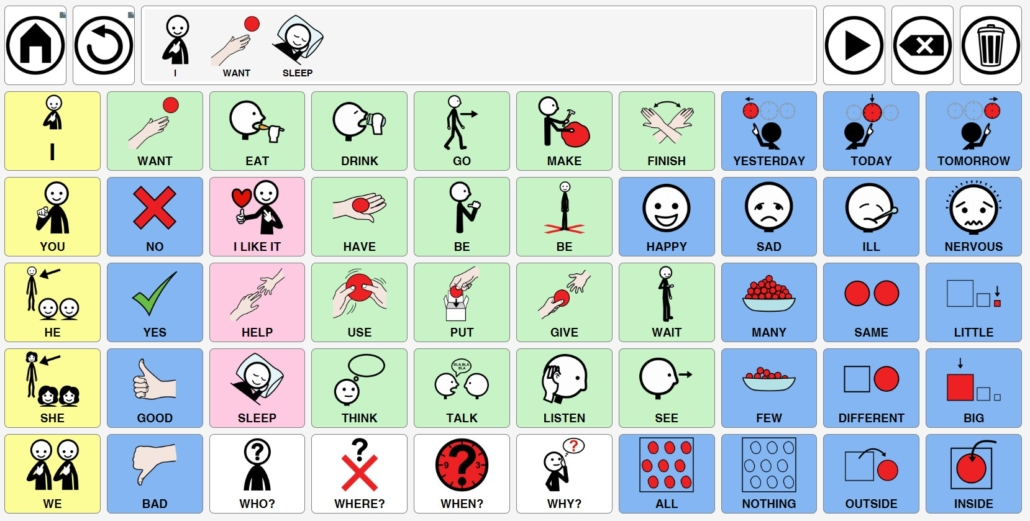
\includegraphics[scale = 0.5]{images/asteriscsGrid.jpg}
\centering
\caption{Comunicador AsTeRISCS Grid desarrollado por ARASAAC}
\end{figure}

Estos pictogramas pueden ser organizados y adaptados dependiendo de las necesidades de cada persona, permitiendo que cada usuario añada aquellos que necesite. El funcionamiento es simple: el usuario clica sobre los pictogramas y el programa se encarga de dar la salida del mensaje, generalmente en forma de habla digitalizada o en formato escrito.

Así, estas herramientas resultan verdaderamente útiles para solventar los problemas de comunicación de las personas. Sin embargo, presentan una limitación que puede afectar a la fluidez y al nivel de expresividad con que se realiza la comunicación: la dificultad para conjugar las frases de manera adecuada, pues para facilitar y simplificar el uso de la herramienta, en este tipo de tableros se suelen incluir solamente palabras clave en su forma simple, sin distinción de número, género o tiempo verbal.

Algunos de los comunicadores que existen actualmente en el mercado ya emplean diferentes métodos para abordar este problema, pero existe todavía un amplio margen de mejora. Los modelos de lenguaje grandes prometen ofrecer buenos resultados en este área.


\section{Objetivos}

Los objetivos de este proyecto son los siguientes:
\begin{enumerate}
\item Investigar sobre los enfoques actuales para la generación de frases en el sector de los SAAC.
\item Implementar y evaluar modelos de lenguaje grandes para este tipo de herramientas.
\item Comparar los resultados que se obtienen con los modelos de lenguaje grandes respecto a otros comunicadores que permiten la generación de frases que se encuentran en el mercado, utilizando para ello las métricas de BLEU y COMET.
\end{enumerate}

\section{Estructura de la memoria}

????? ????????????? ????????????? ????????????? ????????????? ????????????? 

%\section{Notes bibliografiques} %%%%% Opcional

%????? ????????????? ????????????? ????????????? ????????????? ?????????????

%%%%%%%%%%%%%%%%%%%%%%%%%%%%%%%%%%%%%%%%%%%%%%%%%%%%%%%%%%%%%%%%%%%%%%%%%%%%%%%
%                         CAPITOLS (tants com calga)                          %
%%%%%%%%%%%%%%%%%%%%%%%%%%%%%%%%%%%%%%%%%%%%%%%%%%%%%%%%%%%%%%%%%%%%%%%%%%%%%%%

\chapter{Fundamentos}\label{capitulo:fundamentos}

REESCRIBIR: Los modelos de lenguaje se encuadran dentro de las técnicas de procesamiento de lenguaje natural, las cuales forman parte del ámbito del aprendizaje automático. Antes de profundizar en las tareas específicas que realizan los modelos de lenguaje grandes, debemos introducir los conceptos básicos del aprendizaje automático, del aprendizaje profunod y del procesamiento de lenguaje natural. Así, en este capítulo abordaremos las distintas tareas y enfoques del aprendizaje automático, proporcionando el contexto necesario para comprender el funcionamiento y las aplicaciones de los modelos de lenguaje.

\section{Aprendizaje automático}

El aprendizaje automático (en inglés, \textit{machine learning}) es una disciplina dentro de la inteligencia artificial que se centra en el desarrollo y estudio de algoritmos y modelos que permiten que los sistemas puedan relizar tareas específicas sin haber sido explícitamente programados para ello. Este término fue acuñado por Arthur Samuel en el año 1959, quien creo uno de los primeros programas exitosos de esta disciplina, conocido como \textit{the Samuel Ckeckers-playing Program} \cite{samuelCheckers} (el programa de juego de damas de Samuel).

Tom Mitchell \cite{mitchell1997mcgraw} define el proceso de aprendizaje de los programas en el campo del \textit{machine learning} de la siguiente manera:

\textit{"Se dice que un programa aprende de la experiencia $E$ con respecto a alguna clase de tarea $T$, y medida de rendimiento $P$, si su rendimiento en tareas en $T$, medido por $P$, mejora con la experiencia $E$."}

Aunque la idea principal del aprendizaje automático es esta, econtramos diferentes enfoques para el entrenamiento de los algoritmos, dependiendo del tipo de tarea que se quiera llevar a cabo. Estos enfoques son: el aprendizaje supervisado, cuyo objetivo es, a partir de unos datos de entrenamiento, encontrar la función $f$ que realice el mejor mapeo posible entre un conjunto de entradas $X$ y sus salidas correspondientes $Y$, de manera que $(X, Y) = (X, f(Y))$; el aprendizaje no supervisado, que trata de modelar la estructura subyacente de un conjunto de datos para identificar relaciones y patrones, permitiendo así un entendimiento más profundo de los mismos; el aprendizaje semi-supervisado, que cae entre el supervisado y el no supervisado y utiliza una porción de datos etiquetados y no etiquetados y, por último, el aprendizaje por refuerzo, donde el algoritmo aprende a través de retroalimentaciones que va recibiendo, ajustando sus acciones con el objetivo de maximizar una recompensa acumulada a lo largo del tiempo. La tarea principal de este trabajo se realizará utilizando las técincas del aprendizaje supervisado.

Otro concepto importante dentro del aprendizaje automático es el aprendizaje profundo (\textit{deep learning}). El aprendizaje profundo es subconjunto dentro del aprendizaje automático que emplea algoritmos basados en redes neuronales. Dentro de este encontramos métodos como las redes neuronales profundas, las redes neuronales recurrentes, las redes neuronales convulacionales y los transformers, entre otros. Estos métodos tienen aplicaciones significativas en una gran variedad de ámbitos, entre los que se encuentra el procesamiento de lenguaje natural, disciplina en la que se enmarca este trabajo. En las siguientes secciones explicaremos con detalle los conceptos de redes neuronales y transformers.

\section{Redes neuronales}

Las redes neuronales están basadas en el funcionamiento del cerebro humano. Así, igual que en este, las redes neuronales están formadas por miles de billones de neuronas, también llamadas nodos, repartidas en capas. Hay 3 tipos de capas: input, hidden y output layer.

%$https://web.stanford.edu/~jurafsky/slp3/ed3book_jan72023.pdf$
Instead, a modern neural network is a network of small computing units, each
of which takes a vector of input values and produces a single output value. 
Neural networks share much of the same mathematics as logistic regression. But
neural networks are a more powerful classifier than logistic regression, and indeed a
minimal neural network (technically one with a single ‘hidden layer’) can be shown
to learn any function.
The building block of a neural network is a single computational unit. A unit takes
a set of real valued numbers as input, performs some computation on them, and
produces an output.
At its heart, a neural unit is taking a weighted sum of its inputs, with one addibias term tional term in the sum called a bias term. Given a set of inputs x1...xn, a unit has
a set of corresponding weights w1...wn and a bias b, so the weighted sum z can be
represented as:
z = b+
X
i
wixi (7.1)
Often it’s more convenient to express this weighted sum using vector notation; recall
vector from linear algebra that a vector is, at heart, just a list or array of numbers. Thus
we’ll talk about z in terms of a weight vector w, a scalar bias b, and an input vector
x, and we’ll replace the sum with the convenient dot product:
z = w · x+b (7.2)
As defined in Eq. 7.2, z is just a real valued number.
Finally, instead of using z, a linear function of x, as the output, neural units
apply a non-linear function f to z. We will refer to the output of this function as
activation the activation value for the unit, a. Since we are just modeling a single unit, the
activation for the node is in fact the final output of the network, which we’ll generally
call y. So the value y is defined as:
y = a = f(z)


\section{Transformers}

All of these models are based on a technology called Transformers, which was invented by Google Research and Google Brain in 2017. I’ve had trouble finding a good human-readable description of how Transformers work; this is probably the best. [https://learning.oreilly.com/library/view/what-are-chatgpt/9781098152604/ch01.html]

%[https://towardsdatascience.com/transformers-an-overview-of-the-most-novel-ai-architecture-cdd7961eef84]

A Transformer takes some input and generates output. That output might be a response to the input; it might be a translation of the input into another language. While processing the input, a Transformer finds patterns between the input’s elements—for the time being, think “words,” though it’s a bit more subtle. These patterns aren’t just local (the previous word, the next word); they can show relationships between words that are far apart in the input. Together, these patterns and relationships make up “attention,” or the model’s notion of what is important in the sentence—and that’s revolutionary

In itself, attention is a big step forward—again, “attention is all you need.” But Transformers have some other important advantages:

Transformers don’t require training data to be labeled; that is, you don’t need metadata that specifies what each sentence in the training data means. When you’re training an image model, a picture of a dog or a cat needs to come with a label that says “dog” or “cat.” Labeling is expensive and error-prone, given that these models are trained on millions of images. It’s not even clear what labeling would mean for a language model: would you attach each of the sentences above to another sentence? In a language model, the closest thing to a label would be an embedding, which is the model’s internal representation of a word. Unlike labels, embeddings are learned from the training data, not produced by humans.

The design of Transformers lends itself to parallelism, making it much easier to train a model (or to use a model) in a reasonable amount of time.

The design of Transformers lends itself to large sets of training data.

\section{Procesamiento del lenguaje natural}

\section{Modelos de lenguaje grandes (GPT, Gemma, Llama-3)}

%https://learning.oreilly.com/library/view/the-working-limitations/53863MIT65233/chapter001.xhtml#h1-1

Los modelos de lenguaje grandes (en inglés, \textit{Large Language Models} o LLM) son modelos de aprendizaje profundo basados en redes neuronales con miles de millones de parámetros. Estos modelos pueden ser entrenados con grandes cantidades de texto, perimitiéndoles realizar una gran cantidad de tareas en el ámbito del procesamiento de lenguaje natural.

Inicialmente, los LLM operaban de manera secuencial, basando sus predicciones en las distribuciones de probabilidad de las palabras dentro de un texto. Sin embargo, este enfoque tenía la limitación de no considerar el contexto más amplio en el que aparecen las palabras, así como sus distintos significados y asociaciones. Los  avances en la arquitectura de las redes neuronales y, especialmente, la aparición de los transformers, han representado una gran evolución hacia modelos de lenguaje grandes mucho más avanzados, capaces de procesar simultáneamente enormes cantidades de texto y permitiendo establecer relaciones más sólidas entre las palabras y el contexto en que aparecen.

\chapter{Adaptación de modelos de lenguaje grandes (PEFT: LoRA)}

????? ????????????? ????????????? ????????????? ????????????? ????????????? 

\chapter{Resultados experimentales}

\section{Conjunto de datos}

\section{Medidas de evaluación}

\section{Resultados experimentales}

????? ????????????? ????????????? ????????????? ????????????? ?????????????

%%%%%%%%%%%%%%%%%%%%%%%%%%%%%%%%%%%%%%%%%%%%%%%%%%%%%%%%%%%%%%%%%%%%%%%%%%%%%%%
%                                 CONCLUSIONS                                 %
%%%%%%%%%%%%%%%%%%%%%%%%%%%%%%%%%%%%%%%%%%%%%%%%%%%%%%%%%%%%%%%%%%%%%%%%%%%%%%%

\chapter{Conclusions}

????? ????????????? ????????????? ????????????? ????????????? ????????????? 

%%%%%%%%%%%%%%%%%%%%%%%%%%%%%%%%%%%%%%%%%%%%%%%%%%%%%%%%%%%%%%%%%%%%%%%%%%%%%%%
%                                BIBLIOGRAFIA                                 %
%%%%%%%%%%%%%%%%%%%%%%%%%%%%%%%%%%%%%%%%%%%%%%%%%%%%%%%%%%%%%%%%%%%%%%%%%%%%%%%

\begin{thebibliography}{10}

%%%%%%%%%%%%%%%%%%%%%%%%%%%%%%%%%%%%%%%%%%%%%%%%%%%%%%%%%%%%%%%%%%%%%%%%%%%%%%%
% MODEL D'ARTICLE                                                             %
%%%%%%%%%%%%%%%%%%%%%%%%%%%%%%%%%%%%%%%%%%%%%%%%%%%%%%%%%%%%%%%%%%%%%%%%%%%%%%%
\bibitem{light}  %borrar
   Jennifer~S. Light.
   \newblock When computers were women.
   \newblock \textit{Technology and Culture}, 40:3:455--483, juliol, 1999.

\bibitem{samuelCheckers}
	%(2011). Samuel’s Checkers Player. In: Sammut, C., Webb, G.I. (eds) Encyclopedia of Machine Learning. Springer, Boston, MA. https://doi.org/10.1007/978-0-387-30164-8_740

\bibitem{mitchell1997mcgraw}
	Mitchell, Tom M and Learning, Machine
	\newblock McGraw-Hill
	\newblock \textit{New York}, 145--200, 1997

%%%%%%%%%%%%%%%%%%%%%%%%%%%%%%%%%%%%%%%%%%%%%%%%%%%%%%%%%%%%%%%%%%%%%%%%%%%%%%%
% MODEL DE LLIBRE                                                             %
%%%%%%%%%%%%%%%%%%%%%%%%%%%%%%%%%%%%%%%%%%%%%%%%%%%%%%%%%%%%%%%%%%%%%%%%%%%%%%%
\bibitem{ifrah}  %borrar 
   Georges Ifrah.
   \newblock \textit{Historia universal de las cifras}.
   \newblock Espasa Calpe, S.A., Madrid, sisena edició, 2008.

\bibitem{PMLkevinMurphy}
   Kevin P. Murphy
   \newblock \textit{Probabilistic Machine Learning}.
   \newblock Massachusetts Institute of Technology, 2022.

\bibitem{seyedehLeili}
   Seyede Leili Mirtaheri, Reza Shahbazian.
   \newblock \textit{Machine Learning}.
   \newblock CRC Press, septiembre 2022.

%%%%%%%%%%%%%%%%%%%%%%%%%%%%%%%%%%%%%%%%%%%%%%%%%%%%%%%%%%%%%%%%%%%%%%%%%%%%%%%
% MODEL D'URL                                                                 %
%%%%%%%%%%%%%%%%%%%%%%%%%%%%%%%%%%%%%%%%%%%%%%%%%%%%%%%%%%%%%%%%%%%%%%%%%%%%%%%
\bibitem{WAR}
   Comunicat de premsa del Departament de la Guerra, 
   emés el 16 de febrer de 1946. 
   \newblock Consultat a 
   \url{http://americanhistory.si.edu/comphist/pr1.pdf}.

\end{thebibliography}
\cleardoublepage

%%%%%%%%%%%%%%%%%%%%%%%%%%%%%%%%%%%%%%%%%%%%%%%%%%%%%%%%%%%%%%%%%%%%%%%%%%%%%%%
%                           APÈNDIXS  (Si n'hi ha!)                           %
%%%%%%%%%%%%%%%%%%%%%%%%%%%%%%%%%%%%%%%%%%%%%%%%%%%%%%%%%%%%%%%%%%%%%%%%%%%%%%%

\APPENDIX

%%%%%%%%%%%%%%%%%%%%%%%%%%%%%%%%%%%%%%%%%%%%%%%%%%%%%%%%%%%%%%%%%%%%%%%%%%%%%%%
%                         LA CONFIGURACIO DEL SISTEMA                         %
%%%%%%%%%%%%%%%%%%%%%%%%%%%%%%%%%%%%%%%%%%%%%%%%%%%%%%%%%%%%%%%%%%%%%%%%%%%%%%%

\chapter{Configuració del sistema}

????? ????????????? ????????????? ????????????? ????????????? ?????????????

\section{Fase d'inicialització}

????? ????????????? ????????????? ????????????? ????????????? ?????????????

\section{Identificació de dispositius}

????? ????????????? ????????????? ????????????? ????????????? ?????????????

%%%%%%%%%%%%%%%%%%%%%%%%%%%%%%%%%%%%%%%%%%%%%%%%%%%%%%%%%%%%%%%%%%%%%%%%%%%%%%%
%                               ALTRES  APÈNDIXS                              %
%%%%%%%%%%%%%%%%%%%%%%%%%%%%%%%%%%%%%%%%%%%%%%%%%%%%%%%%%%%%%%%%%%%%%%%%%%%%%%%


\chapter{??? ???????????? ????}

????? ????????????? ????????????? ????????????? ????????????? ????????????? 



%%%%%%%%%%%%%%%%%%%%%%%%%%%%%%%%%%%%%%%%%%%%%%%%%%%%%%%%%%%%%%%%%%%%%%%%%%%%%%%
%                              FI DEL DOCUMENT                                %
%%%%%%%%%%%%%%%%%%%%%%%%%%%%%%%%%%%%%%%%%%%%%%%%%%%%%%%%%%%%%%%%%%%%%%%%%%%%%%%

\end{document}
